\documentclass{article}

% Include any necessary packages here
\usepackage{graphicx} % for including figures
\usepackage{amsmath}  % for mathematical symbols and equations
\usepackage{subcaption}
\usepackage{pdfpages}
\usepackage{placeins}

\title{DAG Validity For Astronaut Health}

\author{Maxwell Rehm\thanks{marehm@uci.edu}}

\begin{document}

\maketitle

\begin{abstract}
This is the abstract of your research paper. It should provide a brief summary of your research, including the problem you addressed, the methods used, and the main results.
\end{abstract}

\section{Introduction}

The use of Directed Acyclic Graphs (DAGs) within the Human System Risk Board (HSRB) framework offers a significant advantage in enhancing the outcomes of astronaut missions. By employing DAGs to create knowledge graphs for each of the 30 human system risks NASA tracks, the HSRB aims to foster a shared understanding of causal relationships from spaceflight hazards to mission outcomes. This approach facilitates improved insights and communication among a diverse group of stakeholders, including program managers, systems engineers, operators, and experts from the Human Health and Performance Directorate. 

The PC Algorithm, developed by Peter Spirtes and Clark Glymour, is a graphical algorithm used in the field of causal inference and structural equation modeling. It is designed to discover the causal relationships or causal structure among a set of variables based on observational data. Multiple implementations of the PC Algorithm were tested on diverse datasets involving mice exposed to both real and simulated spaceflight conditions. The primary goal was to assess whether the algorithm could effectively generate Directed Acyclic Graphs (DAGs) to uncover causal relationships within this small-scale, animal-based data. The rationale behind this approach was to evaluate the algorithm's feasibility for later application to human data, given the limited pool of individuals who have ventured into space, making it challenging to establish ground-truth causal relationships.

\section{Methods}

For our experiment, we sourced data from NASA's Open Science Data Repository (OSDR), utilizing a total of eight distinct datasets. We approached data preprocessing with caution, as we aimed to minimize any potential influence or bias on the DAG generation process. The extent of preprocessing varied across these datasets, with a primary objective of maintaining the integrity and fidelity of the original data. Data preperation was necessary to facilitate meaningful comparisons between our DAG results and DAGs manually crafted and verified by domain experts.

\section{Data Sources}

\paragraph{OSD-489 (Dubeé)}

This study involved post-pubescent female C57BL/6J mice subjected to microgravity conditions on the International Space Station (ISS). The mice were euthanized, and their tissues, including lumbar vertebrae (L4), were dissected and assessed for cancellous bone using microcomputed tomography (mCT). The acquired data underwent transformation to align with a microCT data reuse template for efficient data mining, and radiation dosimetry measurements were recorded to account for variations in ionizing radiation exposure during the experiment on the ISS.

Of the original 18 variables measured in the study, we created 3 for ease of interpretation. The \texttt{Expose} variable was created as a boolean indicator, representing whether or not mice were exposed to 37 days of microgravity (microG) flight after transportation to the International Space Station (ISS) and housing in the Rodent Habitat.

Two principal component analyses (PCA) were conducted to extract essential information from the original data. The \texttt{Trab} variable was composed of \texttt{trabecular\_number\_1\_by\_mm} and \texttt{trabecular\_separation\_mm}. A higher trabecular number indicated a denser trabecular bone structure, while lower trabecular separation indicated a more compact and denser trabecular bone configuration.

Similarly, the \texttt{Mass} variable was derived from \texttt{trabecular\_thickness\_m} and \texttt{percent\_bone\_volume\_bvtv\_percent}. Increased trabecular thickness implied stronger and denser trabecular bone, while a larger proportion of bone volume relative to the total tissue volume indicated better bone density and overall bone health. This transformation process helped simplify and focus the dataset, making it more amenable to subsequent analyses and interpretation.


\paragraph{OSD-351 (Keune 2015)}

The study involved the collection of bone-related data from Fischer 344 rats subjected to various conditions, including baseline controls, ground-based flight controls, and actual spaceflight. These rats underwent ovariectomies (OVX) and were sacrificed to analyze bone changes. Micro-computed Tomography (mCT) was used to evaluate bone volume and microarchitecture in different bone segments, such as femora, humeri, lumbar vertebrae, and calvaria, with specific parameters measured for each bone type. Automated contouring was employed to distinguish cortical bone from non-bone material based on gray scale values, and data transformation was applied to align the dataset with a microCT data reuse template for improved data mining. The animal husbandry followed ethical guidelines, with rats assigned to different groups and provided with food and water accordingly.

After data transformations, The dataset includes several variables with specific definitions and measurements. The \texttt{expose} variable is a boolean indicator that specifies whether the subject spent 14 days on Earth or in space, essentially distinguishing between the control and spaceflight groups. \texttt{Mass} is a composite variable derived from \texttt{DXA\_BMC\_mg} and \texttt{DXA\_BMD\_mg\_per\_mmsq}, measuring the change in mass over the 14-day period and was non-invasively measured before and after the experiment.

The \texttt{Meta} category pertains to the metaphysis, which is the transitional region between the shaft (diaphysis) and the rounded end (epiphysis) of a long bone. Within this category, \texttt{mass\_meta} represents the percentage of cancellous bone volume in the metaphysis relative to the total tissue volume in that region. \texttt{Trab\_meta} provides micrometer measurements of the microstructure and density of cancellous bone tissue in the metaphysis region of a bone.

In contrast, the \texttt{Epiphysis} category focuses on the epiphysis, which forms a joint with another bone and represents the rounded end of a long bone. Similar to the metaphysis, \texttt{mass\_epiph} reflects the percentage of cancellous bone volume in the epiphysis relative to the total tissue volume in that region. \texttt{Trab\_epiph} offers micrometer measurements of the microstructure and density of cancellous bone tissue in the epiphysis region of a bone. These variables collectively provide detailed insights into bone characteristics and changes during the experimental period.

\paragraph{OSD-351 (Keune 2016)}

This study involved the collection of data from female Fischer 344 rats, which were subjected to different experimental conditions. The animals were either part of the ground control group or the spaceflight group, with the flight group experiencing 14 days in space on the Space Shuttle Columbia (STS-62). The rats in both groups were housed in animal enclosure modules (AEM) and maintained at 28 °C, with access to food and water ad libitum. Ovariectomies (OVX) were performed on the rats 14 days prior to launch, and their bone characteristics were evaluated using various measurements, including histomorphometry techniques on the second lumbar vertebrae. The collected data underwent a transformation process to align with a standardized bone histomorphometry data template, enabling efficient data mining and analysis.

After further processing, the new dataset encompasses several variables, each with distinct attributes and measurements. The \texttt{expose} variable is a boolean indicator, denoting whether mice participated in a 14-day spaceflight on the Space Shuttle Columbia (STS-62).

Within the dataset, \texttt{resorp} is a composite variable comprising \texttt{Label}\texttt{\_length} \texttt{\_LL}\texttt{\_millimeter}\texttt{\_per}\texttt{\_millimeters}\texttt{\_squared} and \texttt{Osteoclast\_perimeter\_OsCp-} \texttt{eri\_percent}. \texttt{Label\_length\_LL\_millimeter\_per\_millimeters\_squared} quantifies the average length of fluorescent markers (fluorochrome labels) per unit area of bone tissue, providing insights into bone formation and growth rates. \texttt{Osteoclast\_perimeter\_OsCperi\_percent} measures the proportion of osteoclast perimeter (cells responsible for bone resorption) relative to the total bone perimeter, expressed as a percentage.

The \texttt{form} category consists of \texttt{Ceased\_bone\_formation\_CeasedBF\_percent} and \texttt{Mineral\_apposition\_rate\_MAR\_micrometers\_per\_day}. \texttt{Ceased\_bone\_for-} \texttt{mation\_CeasedBF\_percent} indicates the percentage of bone surface where bone formation has halted, highlighting areas where new bone production has ceased. On the other hand, \texttt{Mineral\_apposition\_rate\_MAR\_micrometers\_per\_day} quantifies the rate at which new mineralized bone is added to existing bone tissue daily.

Finally, the \texttt{mass} variable is identical to \texttt{Bone\_volume\_BVTV\_percent}. It assesses the percentage of bone volume relative to the total tissue volume within a specific bone area, offering insights into bone density and composition.

\paragraph{OSD-477, OSD-608 (Ko)}

In OSD-477, after sample collection, the left femur was stored for ex vivo microCT analysis and biomechanical testing, while the right femur was used for dynamic histomorphometry. The femurs were subjected to three-point bending to determine mechanical properties, and microcomputed tomographic (μCT) imaging was performed at specific regions. Image processing involved using global thresholds to evaluate trabecular and cortical bone. Histomorphometry was conducted to assess static and dynamic parameters in trabecular bone. The treatment protocol involved suspending rats at different percentages of their body weight to mimic varying gravitational forces.

In OSD-608, the study involved assessing trabecular and cortical volumetric bone mineral density (vBMD) using in vivo peripheral quantitative computed tomography (pQCT) at the right proximal tibia. The treatment protocol also included suspending rats at different percentages of their body weight to mimic various gravitational forces.

The revised Ko dataset includes various parameters related to skeletal unloading and bone characteristics in rats. The \texttt{unload} parameter is similar to \texttt{PWB} and originally represented the percentage of body weight (20\%, 40\%, 70\%, or 100\%) that rats experienced. However, \texttt{unload} is flipped to represent the percentage of skeletal unloading (80\%, 60\%, 30\%, or 0\%) that rats experienced. The \texttt{dur} parameter represents the duration of skeletal unloading, which could be 1, 2, or 4 weeks (in days).

The \texttt{expose} parameter is a z-score transformation of the product of \texttt{unload} and \texttt{dur}, providing a standardized measure of the combined effect of the extent and duration of skeletal unloading experienced by rats. The \texttt{mass} parameter is composed of \texttt{Bone\_volume\_BV\_per\_total\_volume\_TV\_mm4\_per\_mm4}, which represents the ratio of bone volume (BV) to total tissue volume (TV) in bone tissue, and \texttt{Bone\_mineral\_density\_BMD\_mg\_per\_cubed\_centimeter}, which measures the concentration of minerals in the bone.

The \texttt{trab} parameter is composed of \texttt{Trabecular\_separation\_TbSp\_millime-} \texttt{ter}, representing the average distance between trabeculae in trabecular bone tissue, and \texttt{Trabecular\_number\_TbN\_one\_per\_millimeter}, which counts trabeculae per unit length in trabecular bone tissue. The \texttt{stren} parameter includes \texttt{maximum\_load\_N\_newtons} and \texttt{failure\_load\_newtons}, measuring bone strength.

The \texttt{resorp} parameter, relabeled as \texttt{Osteoclast\_surface\_OcS\_per\_bone\_su-} \texttt{rface\_BS\_percent}, measures the percentage of bone surface covered by osteoclasts, which break down old bone tissue as part of bone remodeling. Lastly, the \texttt{form} parameter is composed of \texttt{Mineralized\_surface\_MS\_per\_bone\_surface\_B-} \texttt{S\_percent}, which measures the percentage of mineralized bone surface, and \texttt{Bone\_formation\_rate\_BFR\_per\_bone\_surface\_BS\_percent}, representing the percentage of bone surface where new bone formation occurs.

Later, the team discussed a plan for concluding the DAG-learning algorithm testing, focusing on the \texttt{Ko} dataset due to its rich variables and known context. They specified two scenarios for running the algorithms on this data. First, they instructed to use only the main \texttt{Ko} dataset (\textit{n}=140) and exclude the \texttt{histo} section. The data should be subset to include observations of either 2 weeks or 4 weeks in duration and animals categorized as either \texttt{PWB100} (no tail suspension/controls) or \texttt{PWB20} (80\% unloaded). A new variable \texttt{unload} should be defined as 0 for the \texttt{PWB100} group and 1 for the \texttt{PWB20} group. This filtering process should result in 44 rows of data. Two scenarios were outlined: "Au naturel," where algorithms would be fed specific variables related to unloading, mass, trabecular measures, and strength; and "PCA-synthetic," where only variables related to unloading, mass (PCA from BVTV and BMD), trabecular (PCA from TbSp and TbN), and strength (PCA from MaxLoad and FailLoad) would be used, excluding duration as it showed little variation in this context. The goal is to observe how algorithms perform under these scenarios in terms of variable relationships.

\paragraph{OSD-366 (Costes)}

In this study, primary fibroblast cells were isolated from the ears of 76 mice from various strains. The mice ears were decontaminated, cut into small pieces, and subjected to collagenase treatment. After incubation, the cells were cultured and expanded, and cells from both male and female mice were used. The irradiation protocol involved exposing the cells to different linear energy transfer (LET) and ion fluence conditions, resulting in various radiation doses. Immunostaining was performed to quantify DNA double-strand breaks, and genotyping was carried out using a high-density SNP array. Data collection included the analysis of two main phenotypes: Background (BGD) and FociPerGray (FPG). BGD represented spontaneous DNA damage, while FPG indicated radiation-induced DNA damage. Significance of SNP-phenotype associations was assessed using statistical tests and corrections for multiple comparisons. Finally, data transformation and analysis were performed using various R packages and tools.

The dataset processing involved filtering to retain only high linear energy transfer (LET) and low LET radiation data while discarding intermediate radiation levels. Subsequently, the data was partitioned by chromosome, ensuring separate datasets for each chromosome. To facilitate further analysis, the chromosome positions within each dataset were one-hot-encoded, creating binary features that represent the presence or absence of each unique chromosome position, enabling efficient handling of genetic information during subsequent analyses.

\paragraph{Consistent Extension}
The pc.stable algorithm, which is commonly used for learning causal structures, often returns CPDAGs, or completed partially directed acyclic graphs. These CPDAGs represent causal relationships among variables, including both directed and undirected edges, reflecting the ambiguity in causal directions. To determine the actual causal directions, we employed bnlearn's cextend() function, which returns an object of class bn representing a DAG, or a directed acyclic graph, that is a consistent extension of the CPDAG obtained from pc.stable. This process involves resolving the undirected edges present in the CPDAG, effectively converting it into a DAG by identifying the causal directions between variables, thus providing a clearer representation of the underlying causal structure.

\section{Results}

\paragraph{OSD-489 (Dubeé)}

The unexpected result of exposure and \texttt{trab} pointing to \texttt{mass} in the algorithm's output suggests a potential deviation from the anticipated causal relationships within the data. In the expected causal structure, \texttt{exposure} should logically influence both \texttt{mass} and \texttt{trab}. However, the algorithm's outcome, with \texttt{expose} and \texttt{trab} pointing to \texttt{mass}, implies that there might be an underlying confounding variable or unaccounted-for factor affecting these relationships.

\begin{figure}[h]
    \begin{minipage}{0.45\textwidth}
        \centering
        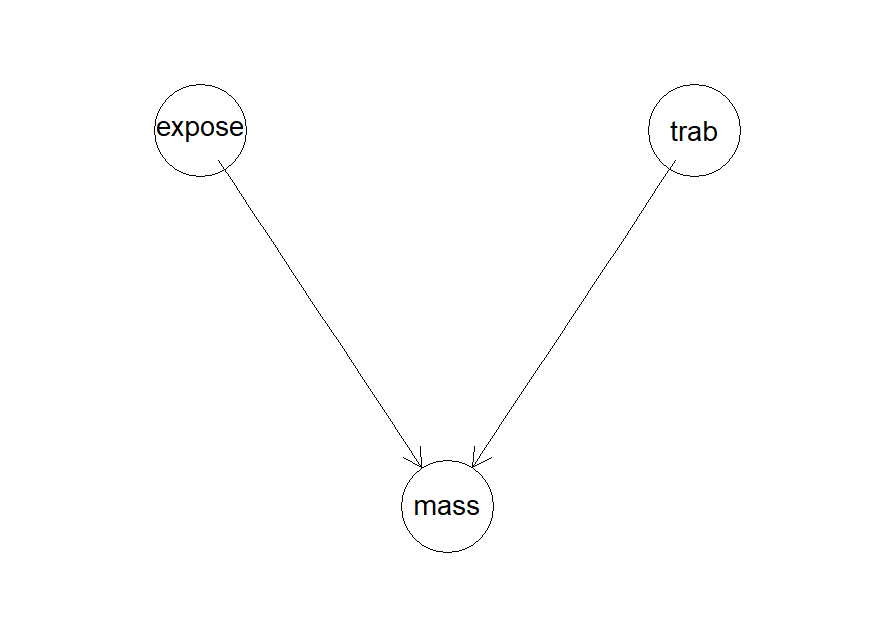
\includegraphics[width=\linewidth]{alwood.png}
        \captionof{subfigure}{pc.stable()}
    \end{minipage}
    \hfill
    \begin{minipage}{0.45\textwidth}
        \centering
        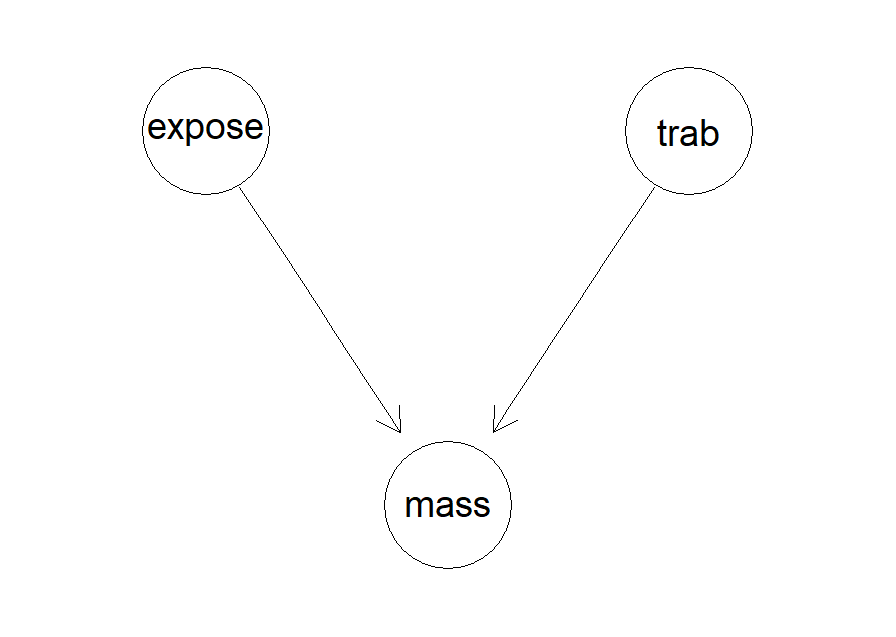
\includegraphics[width=\linewidth]{c_alwood.png}
        \captionof{subfigure}{pc.stable() + cextend()}
    \end{minipage}
\end{figure}
  
\null\newpage




\paragraph{OSD-351 (Keune 2015)}

The observed output, where \texttt{mass\_epiph} points to \texttt{expose} and \texttt{mass} while \texttt{trab\_epiph} remains isolated, and the same result for \texttt{meta}, indicates a divergence from the expected causal relationships in the data. In the anticipated causal structure, \texttt{expose} should logically influence \texttt{trab\_meta} and \texttt{trab\_epiph}, which in turn would affect \texttt{mass}. However, the algorithm's result suggests a disconnect between \texttt{expose} and \texttt{trab\_epiph}, with \texttt{mass\_epiph} directly impacting both \texttt{expose} and \texttt{mass}. This discrepancy could signify unaccounted-for confounding factors or complexities in the data that the algorithm struggles to capture accurately.


\begin{figure}[h] % Use [H] to force figure placement here
    \begin{minipage}{0.45\textwidth}
        \centering
        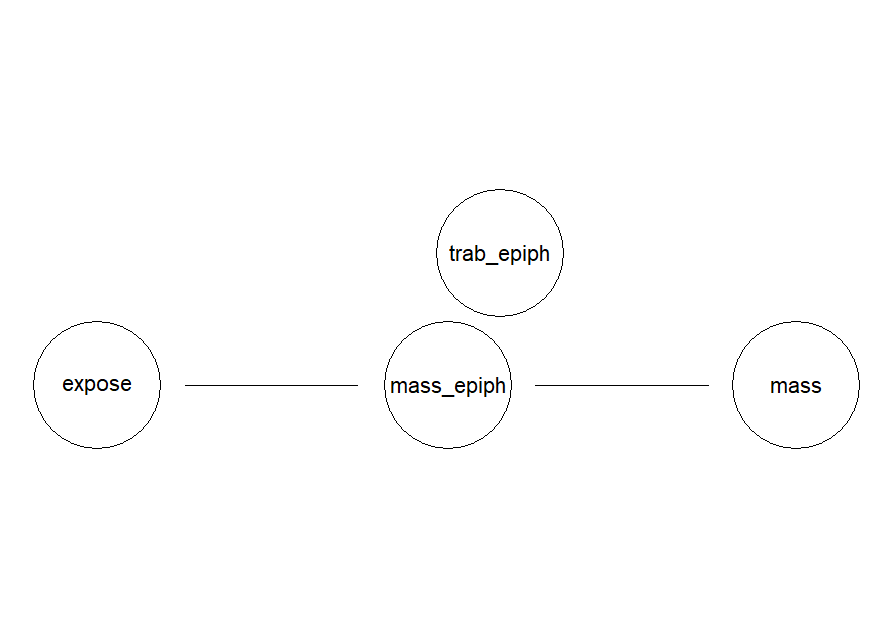
\includegraphics[width=\linewidth]{epiph.png}
        \captionof{subfigure}{pc.stable() of epiphysis group}
    \end{minipage}
    \hfill
    \begin{minipage}{0.45\textwidth}
        \centering
        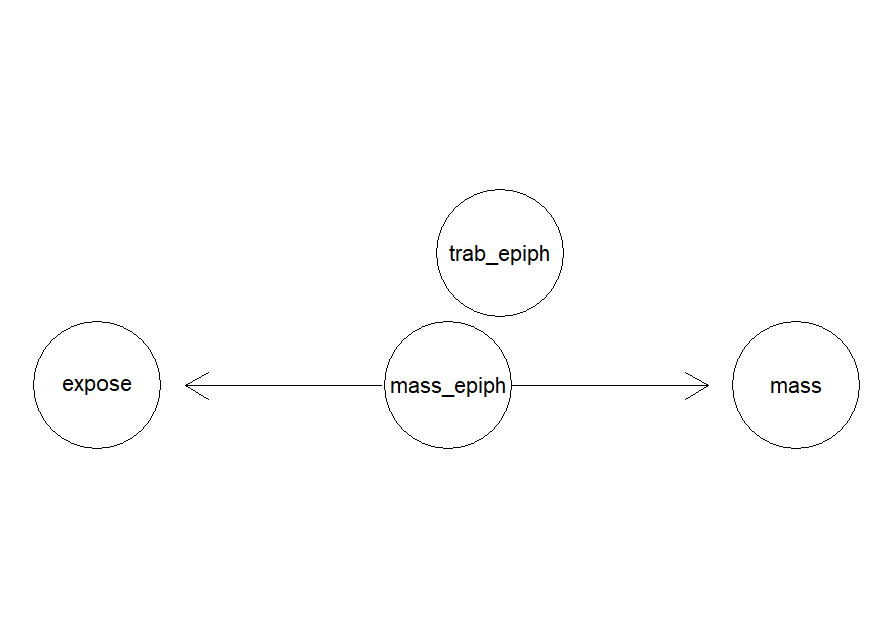
\includegraphics[width=\linewidth]{c_epiph.png}
        \captionof{subfigure}{pc.stable() + cextend() of epiphysis group}
    \end{minipage}
\end{figure}

\begin{figure}[h] % Use [H] to force figure placement here
    \begin{minipage}{0.45\textwidth}
        \centering
        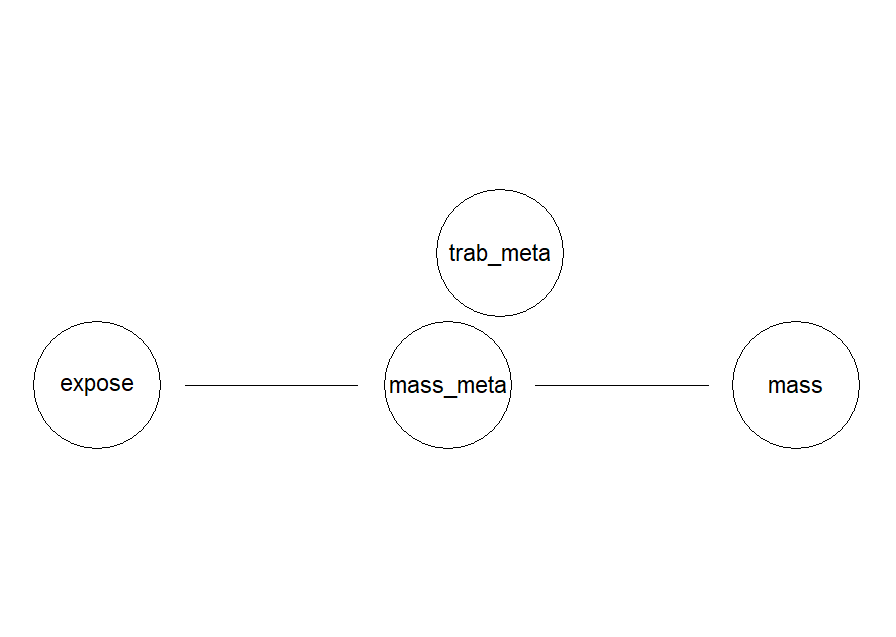
\includegraphics[width=\linewidth]{meta.png}
        \captionof{subfigure}{pc.stable() of metaphysis group}
    \end{minipage}
    \hfill
    \begin{minipage}{0.45\textwidth}
        \centering
        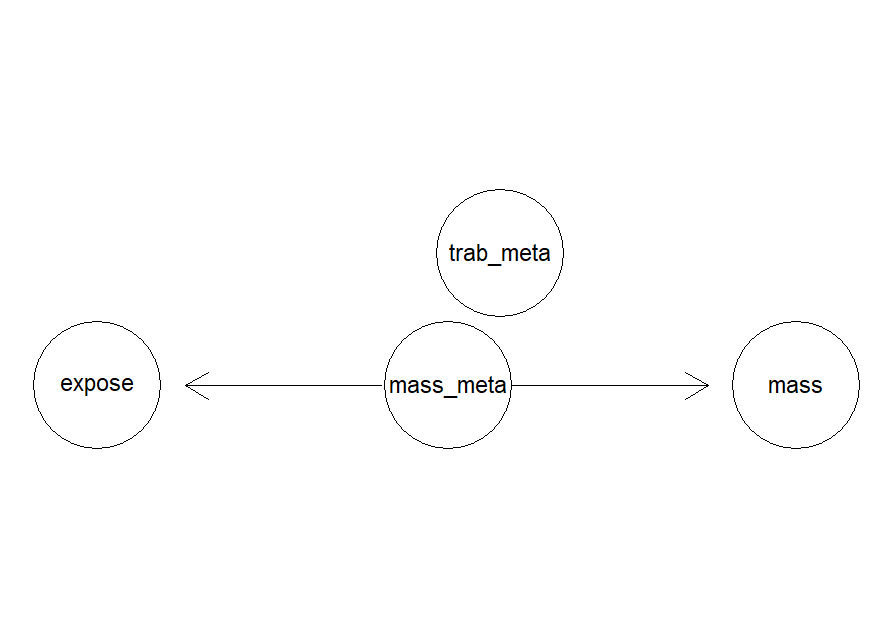
\includegraphics[width=\linewidth]{c_meta.png}
        \captionof{subfigure}{pc.stable() + cextend() of metaphysis group}
    \end{minipage}
\end{figure}


\paragraph{OSD-351 (Keune 2016)}
In this scenario, the expected causal relationship should involve \texttt{expose} influencing \texttt{form} and \texttt{resorp}, with \texttt{form} subsequently impacting \texttt{mass}, and \texttt{resorp} also affecting \texttt{mass}. However, the observed output presents a different picture, where \texttt{resorp} directly influences \texttt{mass}, and surprisingly, \texttt{resorp} seems to influence \texttt{expose}. Notably, the variable \texttt{form} appears to be isolated in this context, which suggests that the algorithm's inferred causal structure deviates from the expected relationships.


\begin{figure}[h] % Use [H] to force figure placement here
    \begin{minipage}{0.45\textwidth}
        \centering
        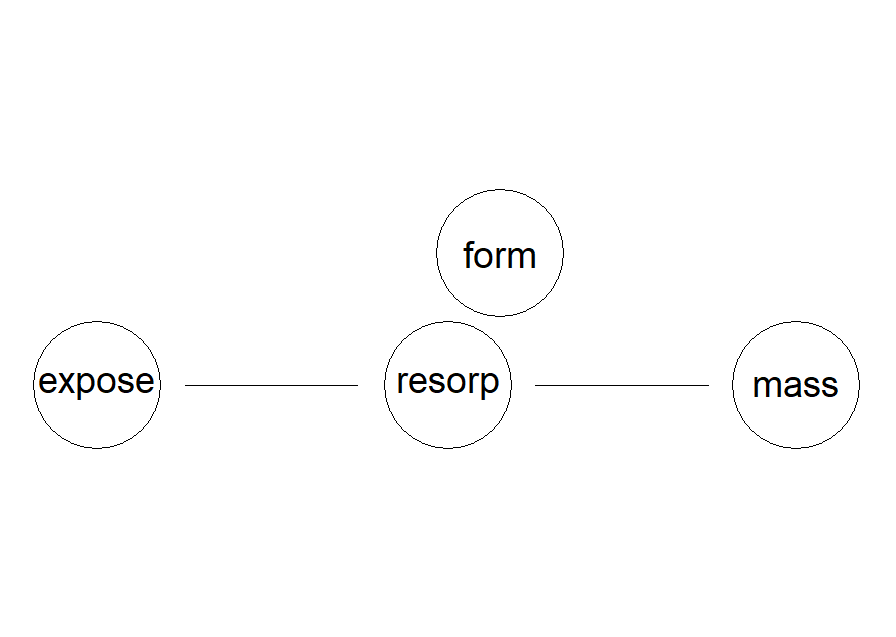
\includegraphics[width=\linewidth]{turner.png}
        \captionof{subfigure}{pc.stable()}
    \end{minipage}
    \hfill
    \begin{minipage}{0.45\textwidth}
        \centering
        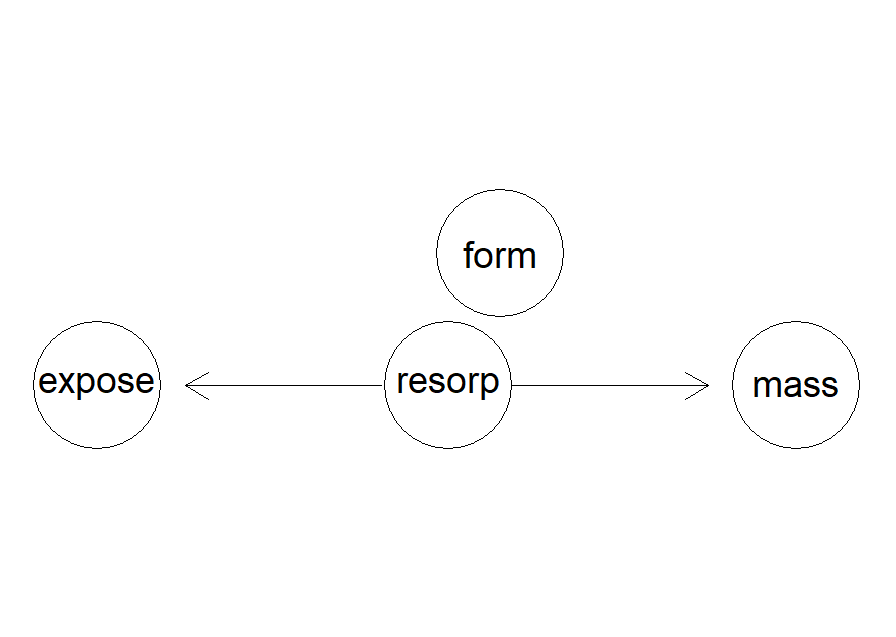
\includegraphics[width=\linewidth]{c_turner.png}
        \captionof{subfigure}{pc.stable() + cextend()}
    \end{minipage}
\end{figure}


\paragraph{OSD-477, OSD-608 (Ko)}

Again, it seems little no meaningful relationships were captured. For the later augmentations, our final attempt, the causal relationships involve unload influencing mass, with mass subsequently affecting strength, and unload also impacting trab, which in turn influences strength. However, the observed output presents a different picture, where mass not only influences strength but is also influenced by unload, suggesting a bidirectional relationship. Similarly, trab and mass exhibit a bidirectional connection, deviating from the expected causal flow

\begin{figure}[h] % Use [H] to force figure placement here
    \begin{minipage}{0.45\textwidth}
        \centering
        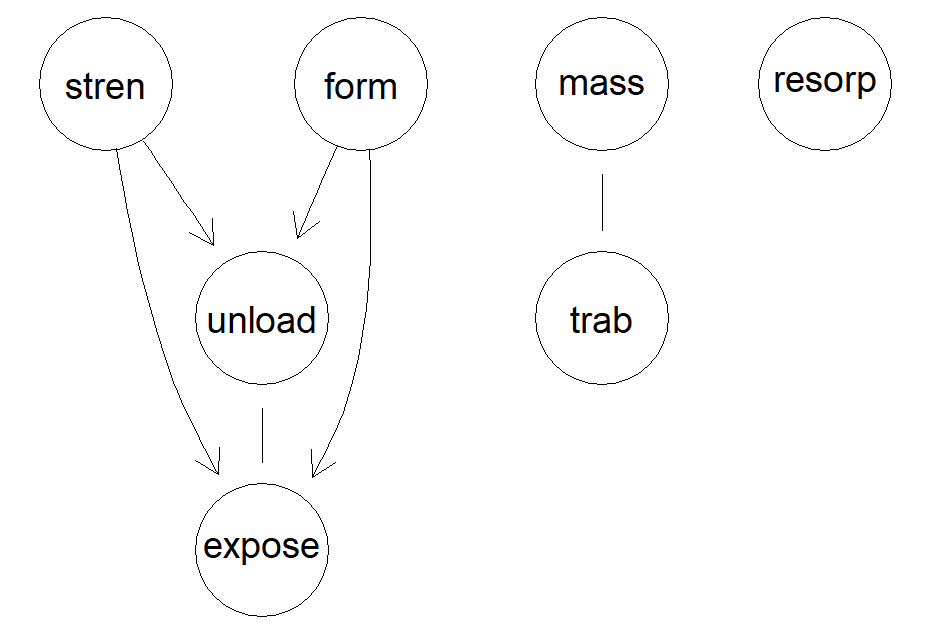
\includegraphics[width=\linewidth]{ko.png}
        \captionof{subfigure}{pc.stable()}
    \end{minipage}
    \hfill
    \begin{minipage}{0.45\textwidth}
        \centering
        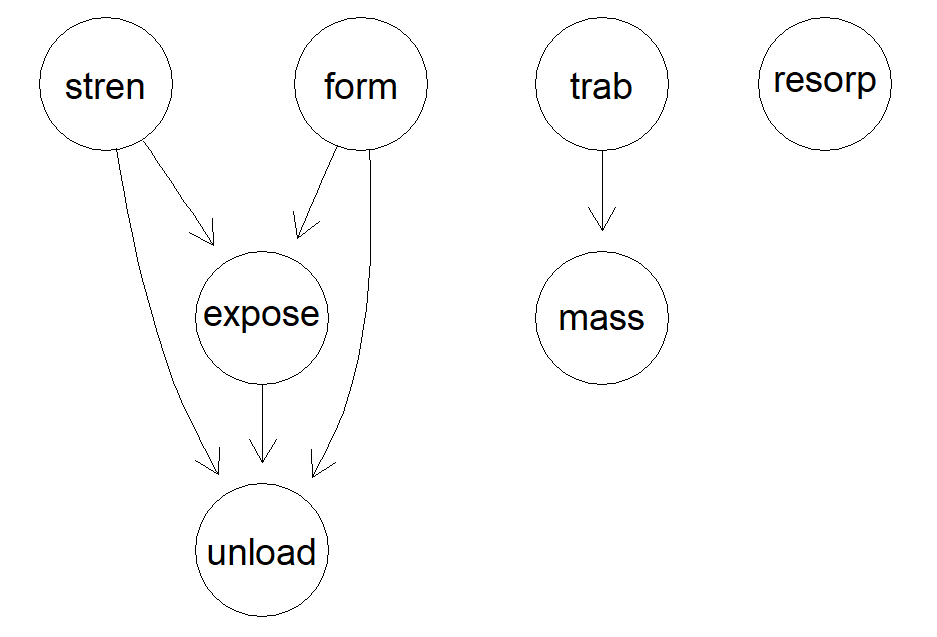
\includegraphics[width=\linewidth]{c_ko.png}
        \captionof{subfigure}{pc.stable() + cextend()}
    \end{minipage}
\end{figure}

\begin{figure}[h] % Use [H] to force figure placement here
    \begin{minipage}{0.45\textwidth}
        \centering
        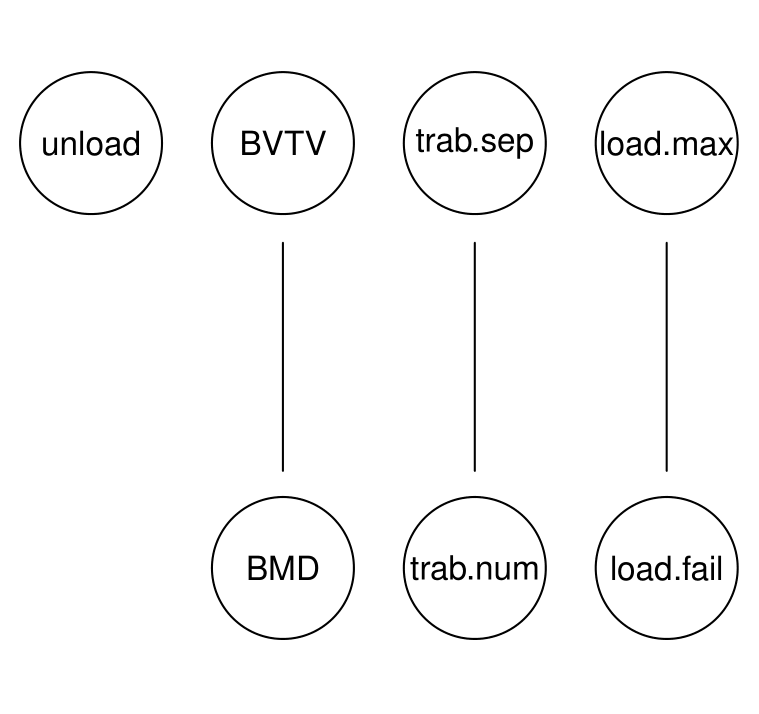
\includegraphics[width=\linewidth]{natural-1.png}
        \captionof{subfigure}{pc.stable() of natural Ko manipualtions}
    \end{minipage}
    \hfill
    \begin{minipage}{0.45\textwidth}
        \centering
        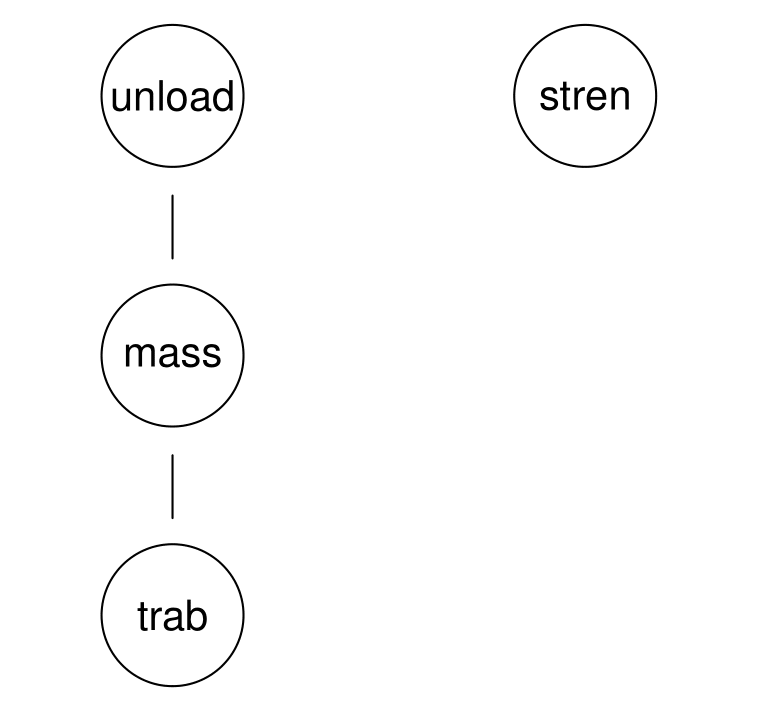
\includegraphics[width=\linewidth]{synthetic-1.png}
        \captionof{subfigure}{pc.stable() of synthetic Ko manipualtions}
    \end{minipage}
\end{figure}


\null\newpage

\paragraph{OSD-366 (Costes)}


The provided data presents intriguing insights into the comparison between high Linear Energy Transfer (LET) radiation (Fe) and low LET radiation (X-ray) by examining the average gap in base pairs. Notably, it demonstrates the effectiveness of causal generation in discerning differences between these radiation types. By quantifying the distances between base pairs, this approach leverages a well-established scientific concept to validate the Directed Acyclic Graphs (DAGs). As indicated in the data, high-LET α-particles, represented by Fe ion radiation, lead to closely interspaced DNA Double-Strand Breaks (DSBs), resulting in high local concentrations of repair proteins. This finding aligns with the established understanding that Fe ion radiation induces more clustered damage compared to X-ray radiation, shedding light on the nuanced impact of different radiation types on DNA.

\begin{table}[ht]
    \centering
    \caption{Top 5 Smallest and Largest Average Gaps (Base Pairs)}
    \begin{tabular}{|l|l|}
    \hline
    \textbf{Name} & \textbf{Average Gap} \\
    \hline
    Fpg\_X.ray\_4 (200) & 55981 \\
    Fpg\_Fe.600.n\_24 (200) & 63652 \\
    Fpg\_Fe.600.n\_8 (100) & 234824 \\
    Fpg\_Fe.600.n\_4 (300 2nd run) & 685386 \\
    Bgd\_Fe.600.n\_8 (100) & 2430299 \\
    \hline
    \end{tabular}
    
    \vspace{10pt} % Add vertical space between the two tables
    
    \begin{tabular}{|l|l|}
    \hline
    \textbf{Name} & \textbf{Average Gap} \\
    \hline
    Bgd\_X.ray\_4 (100) & 263095503 \\
    Bgd\_X.ray\_24 (300 2nd run) & 67767664 \\
    Fpg\_X.ray\_4 (300 2nd run) & 59571718 \\
    Fpg\_X.ray\_48 (300 2nd run) & 53761675 \\
    Fpg\_Fe.600.n\_8 (300 2nd run) & 41168539 \\
    \hline
    \end{tabular}
    \end{table}
    

\null\newpage


\FloatBarrier
\begin{figure}[ht]
  \centering
  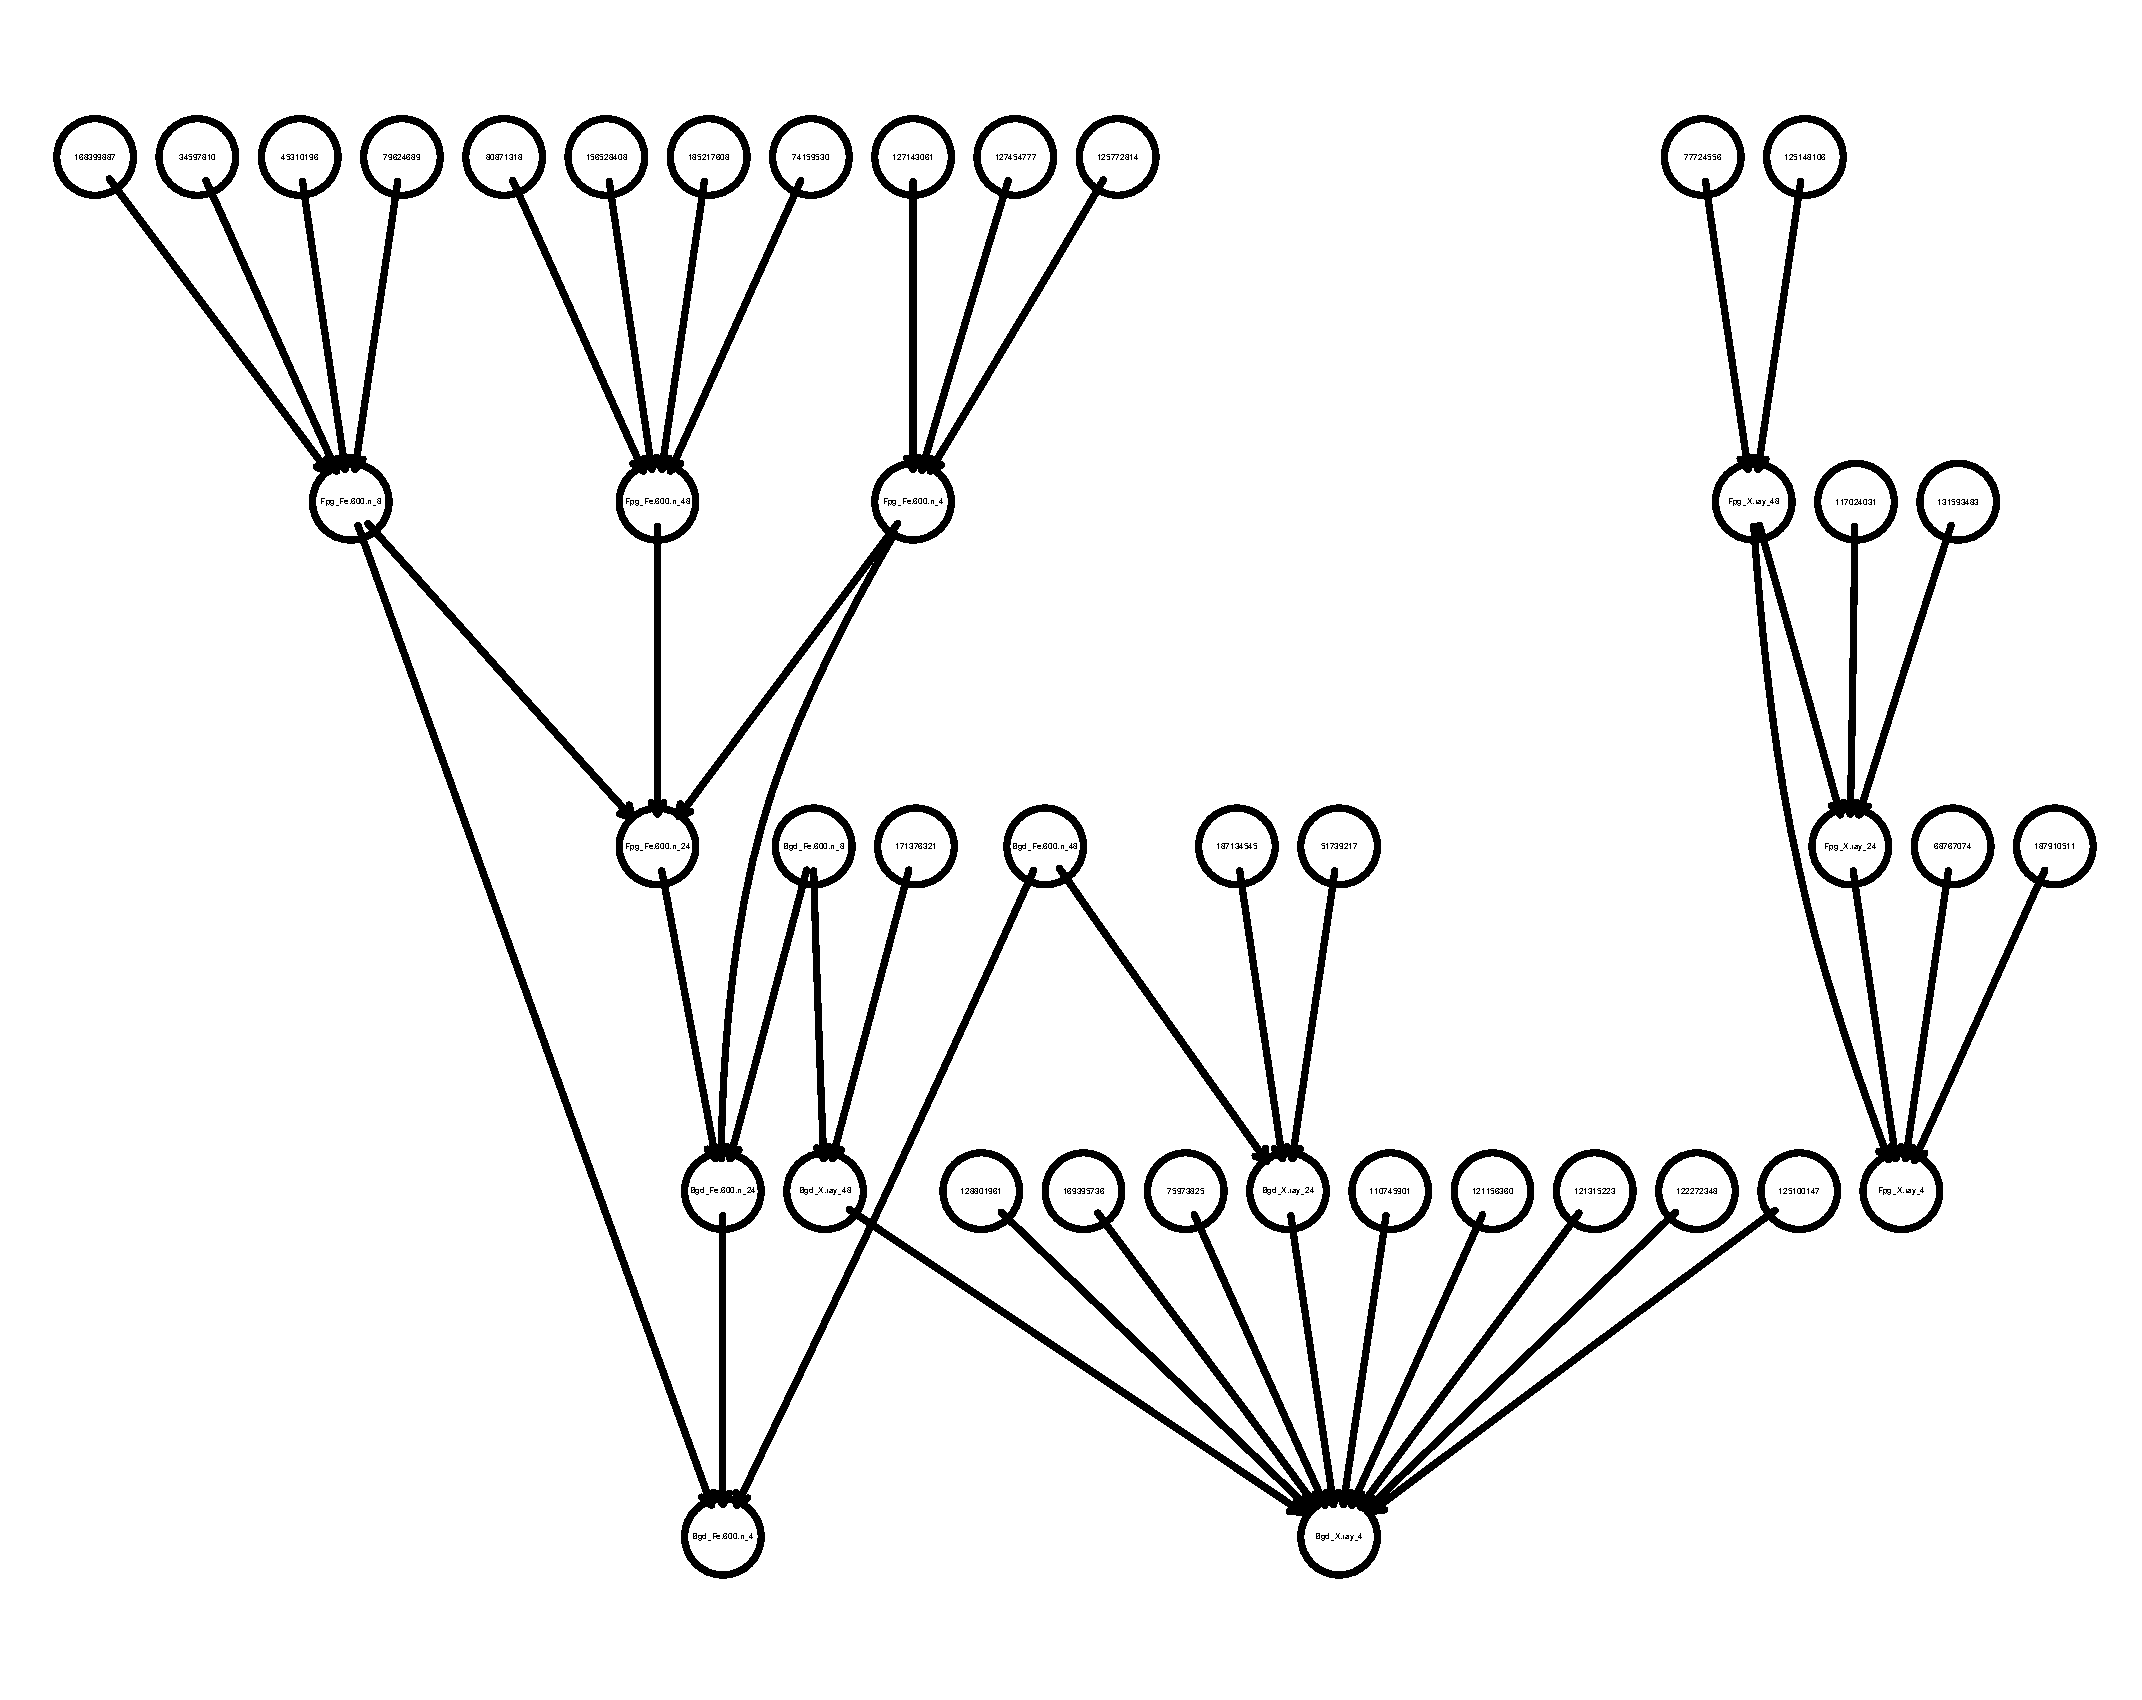
\includepdf[pages=1, scale=0.8]{300 2.pdf}
  \caption{Example run, showing how certain DNA locations cause higher chance of radiation occuring. (300 2nd run from table)}
  \label{fig:your-pdf-figure}
\end{figure}

\null\newpage


\section{Discussion}

In the course of our research, we encountered results that did not meet our initial expectations, prompting us to delve into a thorough discussion of potential factors contributing to these less-than-optimal outcomes. One of the primary considerations is the limitation imposed by the size of our datasets. The availability of extensive and diverse data plays a pivotal role in the success of any machine learning or statistical analysis. In our case, the relatively small dataset at our disposal may have constrained the predictive power of our models and hindered our ability to detect subtle patterns or relationships. This limitation emphasizes the importance of data acquisition and the challenges researchers face when working with constrained resources.

Additionally, it is essential to acknowledge the intricacies and multifaceted nature of the problem we aimed to address. Complex phenomena often require extensive data, sophisticated models, and a comprehensive understanding of underlying variables. Our results may have been influenced by oversimplification or inadequate representation of these complexities within our models.

Furthermore, the choice of algorithms and methodologies is another critical aspect that can significantly impact research outcomes. While we strive to employ state-of-the-art techniques, the selection and parameterization of these methods are inherently subjective and can influence the results. It is essential to continually refine and adapt our approaches to ensure they align optimally with the problem at hand.

Moreover, we cannot discount the potential influence of random variations and noise within the data. In relatively small datasets, the impact of outliers or noisy data points can be disproportionately significant, leading to unexpected results. Robust preprocessing and data cleansing techniques are essential to mitigate such issues.

\section{Conclusion}

In conclusion, our research journey has revealed valuable insights into the complexities of data analysis and the challenges that researchers often encounter. Despite encountering less-than-ideal results, we recognize that these outcomes provide opportunities for growth and learning. The limitations posed by small datasets, the intricacies of the problem under investigation, and the influence of various factors on our models are all valuable lessons that will inform our future research efforts. As we move forward, we remain committed to refining our methodologies, expanding our data resources, and enhancing the robustness of our analyses. Through perseverance and continuous improvement, we are confident in our ability to contribute meaningfully to the field of data analysis and machine learning.

\section*{Acknowledgments}

I would like to express my heartfelt gratitude to the University of California, Irvine, for providing a conducive environment for academic growth and research. Special thanks to Nadia Ahmed for her instrumental role in introducing me to this project, and to Lauren Sanders for her invaluable biological insights and support throughout the research journey. I am deeply thankful to Ryan Scott, Robert Reynolds, and Sylvain Costes for their guidance and expertise in navigating the intricacies of Directed Acyclic Graphs (DAGs). Last but not least, I would like to acknowledge the contributions of Elias Eulig for their assistance in the realm of DAGs. Your collective efforts have significantly enriched this research endeavor.


\end{document}
